% Document layout
\documentclass[a4paper,12pt]{article}
\usepackage[left=15mm, right=15mm, top=25mm, bottom=20mm]{geometry}

% \usepackage[utf8]{inputenc} % XeLaTeX doesn't need it!

% Bibliography
\usepackage[backend=biber,style=ieee]{biblatex}
\addbibresource{references.bib}

% Font
\usepackage{fontspec}
\setmainfont{TeX Gyre Termes}

% Indentation
% \setlength\parindent{0pt}
% \usepackage{indentfirst}

%Hyperlinks, Graphs and formatting
\usepackage[colorlinks,allcolors=black]{hyperref}
\usepackage{float}
\usepackage{graphicx}
\usepackage{multicol}
\setlength{\columnsep}{1cm}

% Color links
% \usepackage[colorlinks,allcolors=blue]{hyperref}

% Title
\usepackage{titling}
\setlength{\droptitle}{-3em}
\title{
\textbf{Multiple Vessel Detection and Tracking in Harsh Maritime Environments}
}
\author{
    Nicholas Hopf\\
    %\small\textit{Faculty of Engineering}\\\small\textit{University of Porto}\\
    up200000000
    \and
    Rodrigo Gomes\\
    %\small\textit{Faculty of Engineering}\\\small\textit{University of Porto}\\
    up201800163
    \and
    Rui Colaço\\
    %\small\textit{Faculty of Engineering}\\\small\textit{University of Porto}\\
    up200000000
}
\date{\vspace{-3ex}}

% Fancy header
\usepackage{fancyhdr}
\usepackage{color}
\fancypagestyle{plain}{\pagestyle{fancy}}
\thispagestyle{fancy}
\pagestyle{fancy}
\fancyhf{}
\fancyhead[R]{Computer Vision Project Report}
\fancyhead[L]{May 2023}
% \fancyfoot[L]{\textit{Faculty of Engineering - University of Porto}}
\fancyfoot[R]{Page \thepage}
\setlength{\headheight}{16pt}

%---------------------------------------------------------

\begin{document}

\maketitle


\vspace{10pt}

\begin{table}[h]
	\centering
	\begin{tabular}{p{14cm}}
        % TODO: Revisar
        {\textbf{Abstract:}} This project focuses on the detection and tracking of vessels in a maritime environment using computer vision techniques.
        The goal is to develop a robust tracking model for Autonomous Surface Vehicles (ASVs) that can effectively handle the challenges posed by harsh environmental conditions.
        The project leverages the research work presented in the paper titled ``Multiple Vessel Detection and Tracking in Harsh Maritime Environment''~\cite{MVDTHME} as a guide for strategies and results.
        The proposed approach combines transfer learning techniques based on YOLO-v8 for object detection and the DeepSORT algorithm for motion tracking.
        The PyTorch framework is utilized for neural network training.
        The project utilizes two datasets, namely the Singapore Maritime Dataset~\cite{SINGAPORE} for training and evaluating object tracking tests, and the Extended MARVEL Dataset~\cite{MARVEL} for training the classifier in the tracking module.
        By addressing the challenges of vessel detection and tracking in real-time and dynamic maritime scenarios, this project contributes to the advancement of computer vision research initiatives in the field of ASV navigation and collision avoidance.
	\end{tabular}\label{tab:abstract}
\end{table}

\begin{multicols}{2}

\section{Introduction and State of the Art}\label{sec:introduction-and-state-of-the-art}
% TODO: %Revisar
The ability of ASVs to operate autonomously in maritime environments holds great potential for applications in various domains such as surveillance, maritime transportation, and environmental monitoring.
However, the reliable detection and tracking of vessels in such environments remains a critical challenge, particularly in the presence of dynamic obstacles and complex lighting conditions.

To address these challenges, this project aims to develop a vessel detection and tracking system for ASVs using computer vision techniques.
The work builds upon the research presented in the paper titled ``Multiple Vessel Detection and Tracking in Harsh Maritime Environment''~\cite{MVDTHME}, which provides valuable insights into strategies and results related to this specific problem domain.
The guidance provided by professors Andry Pinto and Daniel Campos, renowned experts in computer vision and associated research initiatives at FEUP and INESC TEC, ensures that the project aligns with ongoing research efforts.

The primary focus of this project is to enhance collision avoidance capabilities in ASVs by accurately detecting and tracking neighboring vessels in real-time.
The maritime environment introduces unique challenges, including vessel motion, changing lighting conditions, and harsh weather.
Therefore, the proposed tracking model needs to demonstrate robustness and reliability even in adverse conditions.

To achieve this, the project leverages transfer learning techniques based on YOLO-v8, a state-of-the-art object detection framework, for vessel detection.
Transfer learning allows the model to leverage pre-trained neural networks on large-scale datasets, significantly reducing the training time and improving performance.
The detection module will be trained using the Singapore Maritime Dataset, which provides videos accompanied by matrix files containing bounding box annotations for vessels in each frame.

To enable motion tracking, the project employs the DeepSORT algorithm, which combines deep learning-based detection with the SORT algorithm for data association.
DeepSORT utilizes temporal information to improve tracking accuracy and handles occlusions and temporary disappearances of vessels.
The tracking module's classifier will be trained using the MARVEL Dataset, which comprises a diverse collection of vessel images across different classes.

PyTorch, a popular deep learning framework, will be utilized for all tasks related to neural network training, providing a flexible and efficient environment for model development and evaluation.

By developing a reliable vessel detection and tracking system, this project contributes to the advancement of computer vision research initiatives in ASV navigation and collision avoidance.
The outcome will be a valuable asset for improving the safety and efficiency of autonomous maritime operations, with potential applications in various domains, including maritime surveillance, search and rescue, and marine transportation.

\section{Dataset}\label{sec:dataset}
% TODO: %%Revisar
The project leveraged the use of two datasets, the Extended MARVEL Dataset~\cite{MARVEL} and the Singapore Maritime Dataset~\cite{SINGAPORE}.

The MARVEL Dataset is a comprehensive collection of images specifically designed for training the classifier in the tracking module of the vessel detection and tracking system.
The dataset consists of a vast repository of 100,000 images showcasing different vessels from various viewpoints and perspectives.
The images are carefully distributed over 38 distinct vessel classes, representing a wide range of maritime vessels, including cargo ships, fishing boats, sailboats, and more.
The dataset provides a rich variety of vessel types, enabling the development of a highly accurate and robust classifier.

The Singapore Maritime Dataset is a comprehensive collection of videos specifically curated for training and evaluating object tracking tests in a maritime environment.
The dataset provides a realistic representation of vessels in various scenarios, capturing the complexity and challenges of real-world maritime operations.
The 81 videos, which, in total, have a size of 5278 Mb, encompass diverse lighting conditions, vessel types, and dynamic movements, making it an ideal resource for developing robust object tracking algorithms.
Each video in the dataset is accompanied by matrix files that contain bounding box annotations for every object present in each frame.
These annotations enable precise ground truth information for evaluation and performance analysis.
By leveraging this data, the project aims to improve the vessel classification component of the tracking module, enhancing the overall performance and reliability of the vessel detection and tracking system.

\section{Methodology}\label{sec:methodology}
% TODO: Revisar
Our objective was to replicate and expand the work done in the original paper~\cite{MVDTHME}, making it possible to identify classes of ships, which was one of the main focuses of the project since it is an important aspect that was not implemented, and track them along their route.

\hfill\newline
Write the stuff mentioned in the proposal\ldots % TODO
\hfill\newline

Given a new video, our model should properly track and classify each maritime vehicle in frame.

To achieve such result, the process :
\begin{enumerate}
    \item \textbf{get frames} from the input video
    \item \textbf{detect} boats from each frame with YOLO, computing their classes and bounding boxes
    \item \textbf{track} boats with DeepSORT~\cite{DEEPSORT} given a list of bounding boxes and their classes
\end{enumerate}

To train the model we obtained one image for every N seconds in each video from the Singapore Maritime Dataset~\cite{SINGAPORE}

Beyond the common augmentation techniques already included in the YOLO training process, we also applied histogram correction and sharpening to augment the data and minimize exposure issues that are sometimes present in the images.
We used the Extended MARVEL Dataset~\cite{MARVEL} to train the classifier in the tracking model.

% TODO: Revisar
The evaluation metric used in this study is Mean Average Precision (mAP), which serves as a measure to compare the accuracy of different training exercises.
The mAP calculation involves assessing the precision of detections for each class of objects in the dataset.
Initially, the focus is on mAP with an Intersection over Union (IoU) threshold of more than 50\%.
This threshold determines the overlap between predicted bounding boxes and ground truth boxes.
By calculating the average precision at this IoU threshold, the performance of the models can be evaluated based on their ability to accurately detect objects.

\section{Results and Analysis}\label{sec:results-and-analysis}

% TODO: Texto e dados baseados no paper, revisar e trocar para os dados dos experimentos
The evaluation results are presented in tables, showcasing the measured mAP@.5 values for different optimizers such as Adam, Adadelta, and SGD. The performance of each optimizer is analyzed, considering various combinations of learning rates and momenta.
The Adam and Adadelta optimizers consistently achieve mAP@.5 scores above 80\%, as demonstrated in the original paper~\cite{MVDTHME}, with the Adam optimizer performing best with a learning rate of 0.001 and momentum of 0.8. The SGD optimizer, while inferior in performance, still demonstrates some results that are comparable to the other optimizers.

% TODO: mAP50 is the mean Average Precision at a 50\% IoU (Intersection over Union) threshold.
\begin{figure}[H]
    \centering
    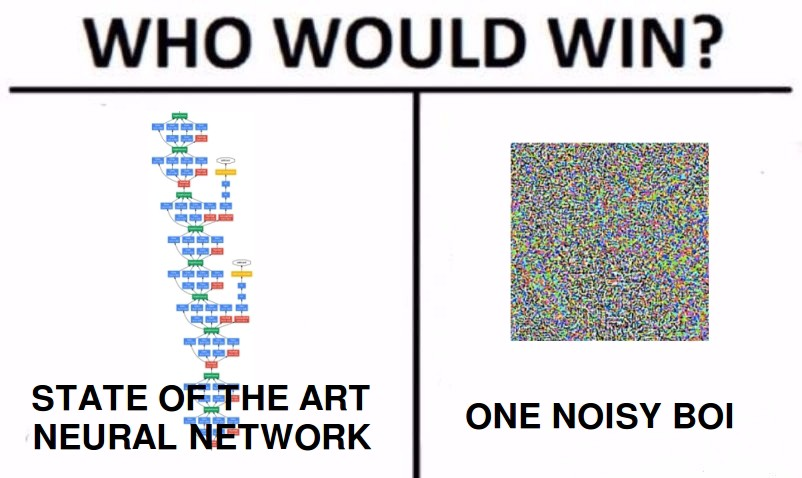
\includegraphics[width=0.45\textwidth]{placeholder}
    \caption{Placeholder text}
    \label{fig:1}
\end{figure}

The evolution of the mAP[.5:.95] metric is examined to gain insights into the quality of detections throughout the training process.
This metric measures the average mAP at different IoU thresholds, ranging from 0.5 to 0.95 with a step size of 0.05.
By observing the evolution of mAP[.5:.95], it becomes apparent that there is a 3.8\% improvement when comparing the performance of Adadelta and Adam optimizers.
The mAP[.5:.95] metric provides a more comprehensive evaluation of the models, considering a range of IoU thresholds and highlighting their ability to accurately detect objects with higher overlap.

\begin{figure}[H]
    \centering
    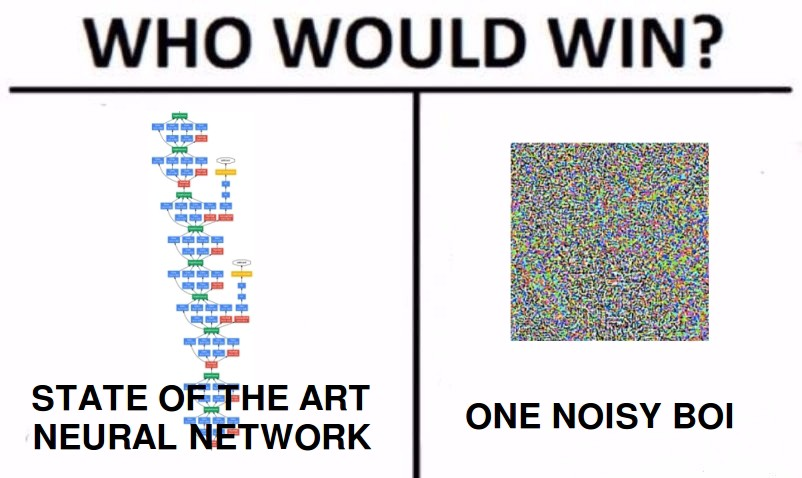
\includegraphics[width=0.45\textwidth]{placeholder}
    \caption{Placeholder text}
    \label{fig:2}
\end{figure}


% TODO: Inserir tracking results

% TODO: Revisar
The use of the MARVEL extended dataset for training instead of the MARVEL micro, since it has a broader and more encompassing representation of scenarios and ships, leads to better classification and performance in real-world maritime events, but, as the dataset is considerably larger, it takes a greater amount of computing power to process, leading to a possible analysis between cost and benefit in the study. Below there is a graph for the classification of the images comparing the results of the model trained with the different datasets:

\begin{figure}[H]
    \centering
    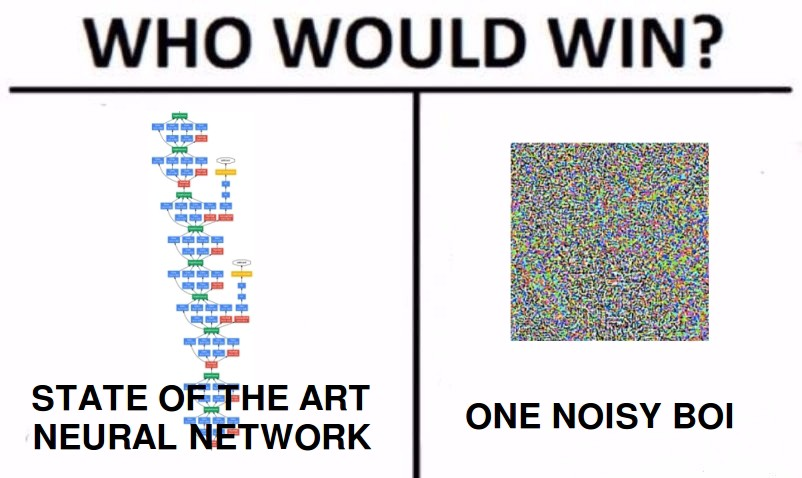
\includegraphics[width=0.45\textwidth]{placeholder}
    \caption{Placeholder text}
    \label{fig:3}
\end{figure}

\section{Opportunities}\label{sec:opportunities}
% TODO: revisar
Some cases of anchor overlapping were identified in the implementation described above.
It is possible to perform ``Non-Maximum Suppression'' or change the applied method, resorting to an anchor-free tracking approach.
In March 2023 Yantong \textit{et al.}~\cite{FAIRMOT} obtained successful tracking results with the Singapore Maritime Dataset while working with FairMOT and Deep Layer Aggregation (DLA) instead of DeepSORT and YOLO\@.
Another option for exploration would be resorting to the recently published StrongSORT~\cite{STRONGSORT} tracker.

\section{References}\label{sec:references}
\printbibliography
\end{multicols}
\end{document}
